\chapter*{ANTON-BIVENS-DAVIS 9.7 EJERCICIO 30}
\textbf{30)} Encuentra los primeros 4 polinomios distintos de Taylor sobre $x = x_{0}$, y usa una utilidad gráfica para graficar la función dada y el polinomio de Taylor en la misma pantalla. \\
\begin{center}
   $f(x) = ln(x+1)$ en $  x_{0}= 0$
\end{center}
Para facilitar la búsqueda de estos polinomios, primero hallemos las derivadas:
\begin{multicols}{3}
	\noindent
	\begin{align*}
		\text{Derivando: } &        \\
		f^{0}(x) =& ln(x+1) \\
        f^{1}(x) =& \frac{1}{x+1} \\
        f^{2}(x) =& -\frac{1}{(x+1)^{2}} \\
        f^{3}(x) =& \frac{2}{(x+1)^{3}} \\
	\end{align*}
	\columnbreak
	\begin{align*}
		\text{Evaluando en: }& x_{0} = 0     \\
		f^{0}(0) =& ln(1) \\
        f^{1}(0) =& \frac{1}{1} \\
        f^{2}(0) =& -\frac{1}{(1)^{2}} \\
        f^{3}(0) =& \frac{2}{(1)^{3}} \\
	\end{align*}
	\columnbreak
	\begin{align*}
		\text{Valor: }&      \\
        ln(1)              =& 0 \\
        \frac{1}{1}        =& 1 \\
        -\frac{1}{(1)^{2}} =&-1 \\
        \frac{2}{(1)^{3}}  =& 2 \\
	\end{align*}
\end{multicols}
Para generar los diferentes polinomios y dado que $x_{0} = 0$, utilizaremos el desarrollo de Mclaurin.
\begin{align*}
   \sum_{k=0}^{n} \frac{f^{k}(0)}{k!}(x)^{k}
\end{align*}
Para $P_{0}(x)$ :
\begin{align*}
   \sum_{k=0}^{0} \frac{f^{k}(0)}{k!}(x)^{k} &= \frac{f^{0}(0)}{0!}(x)^{0} \\
   \frac{f^{0}(0)}{0!}(x)^{0} &= \frac{ln(0+1}{0!}(x)^{0}\\
   \frac{ln(0+1}{0!}(x)^{0} &= \frac{8}{1}(1)\\
\end{align*}
Así, esta es nuestra \textbf{primera} aproximación a la función. $P_{0}(x) = 0$ \\

Para $P_{1}(x)$ :
\begin{align*}
   \sum_{k=0}^{1} \frac{f^{k}(0)}{k!}(x)^{k} &= \frac{f^{0}(0)}{0!}(x)^{0} + \frac{f^{1}(0)}{1!}(x)^{1} \\
\end{align*}
Para el nuevo Término:
\begin{align*}
   \frac{f^{1}(0)}{1!}(x)^{1}                    &= \frac{\frac{1}{0+1}}{1}x^{1} \\
   \frac{\frac{1}{0+1}}{1}x^{1}                  &= \frac{1}{1}x^{1} \\
   \frac{1}{1}x^{1}                              &= x \\
\end{align*}
Así la sumatoria resulta:
\begin{align*}
   \sum_{k=0}^{1} \frac{f^{k}(0)}{k!}(x)^{k} &= 0 + x\\
\end{align*}
Así, esta es nuestra \textbf{segunda} aproximación a la función. $P_{1}(x) = 0 + x$ \\


Para $P_{2}(x)$ :
\begin{align*}
   \sum_{k=0}^{2} \frac{f^{k}(0)}{k!}(x)^{k} &= \frac{f^{0}(0)}{0!}(x)^{0} + \frac{f^{1}(0)}{1!}(x)^{1}  + \frac{f^{2}(0)}{2!}(x)^{2}\\
\end{align*}
Para el nuevo Término:
\begin{align*}
   \frac{f^{2}(0)}{2!}(x)^{2}                   &= \frac{-\frac{1}{(0+1)^{2}}}{2!}x^{2} \\
   \frac{-\frac{1}{(0+1)^{2}}}{2!}x^{2}         &= \frac{-\frac{1}{1}}{2}x^{2} \\
   \frac{-\frac{1}{1}}{2}x^{2}                  &= \frac{-1}{2}x^{2}  \\
   \frac{-1}{2}x^{2}                            &= -\frac{x^{2}}{2}\\
\end{align*}
Así la sumatoria resulta:
\begin{align*}
   \sum_{k=0}^{2} \frac{f^{k}(0)}{k!}(x)^{k} &= 0 + x -\frac{x^{2}}{2}\\
\end{align*}
Así, esta es nuestra \textbf{tercera} aproximación a la función. $P_{2}(x) = 0 + x -\frac{x^{2}}{2}$ \\

Para $P_{3}(x)$ :
\begin{align*}
   \sum_{k=0}^{3} \frac{f^{k}(0)}{k!}(x)^{k} &= \frac{f^{0}(0)}{0!}(x)^{0} + \frac{f^{1}(0)}{1!}(x)^{1} + \frac{f^{2}(0)}{2!}(x)^{2} + \frac{f^{3}(0)}{3!}(x)^{3}\\
\end{align*}
Para el nuevo Término:
\begin{align*}
   \frac{f^{3}(0)}{3!}(x)^{3}                   &= \frac{\frac{2}{(0+1)^{3}}}{3!}x^{3} \\
   \frac{\frac{2}{(0+1)^{3}}}{3!}x^{3}         &= \frac{\frac{2}{1}}{3!}x^{3} \\
   \frac{\frac{2}{1}}{3!}x^{3}                  &= \frac{2}{6}x^{3}  \\
   \frac{2}{6}x^{3}                            &= \frac{x^{3}}{3}\\
\end{align*}
Así la sumatoria resulta:
\begin{align*}
   \sum_{k=0}^{3} \frac{f^{k}(0)}{k!}(x)^{k} &= 0 + x -\frac{x^{2}}{2} + \frac{x^{3}}{3}\\
\end{align*}
Así, esta es nuestra \textbf{cuarta} aproximación a la función. $P_{3}(x) = 0 + x -\frac{x^{2}}{2} + \frac{x^{3}}{3}$ \\

\textbf{A continuación están las gráficas, tanto de la función original como de los Polinomios Generados:} \\

\begin{figure*}
    \centering
    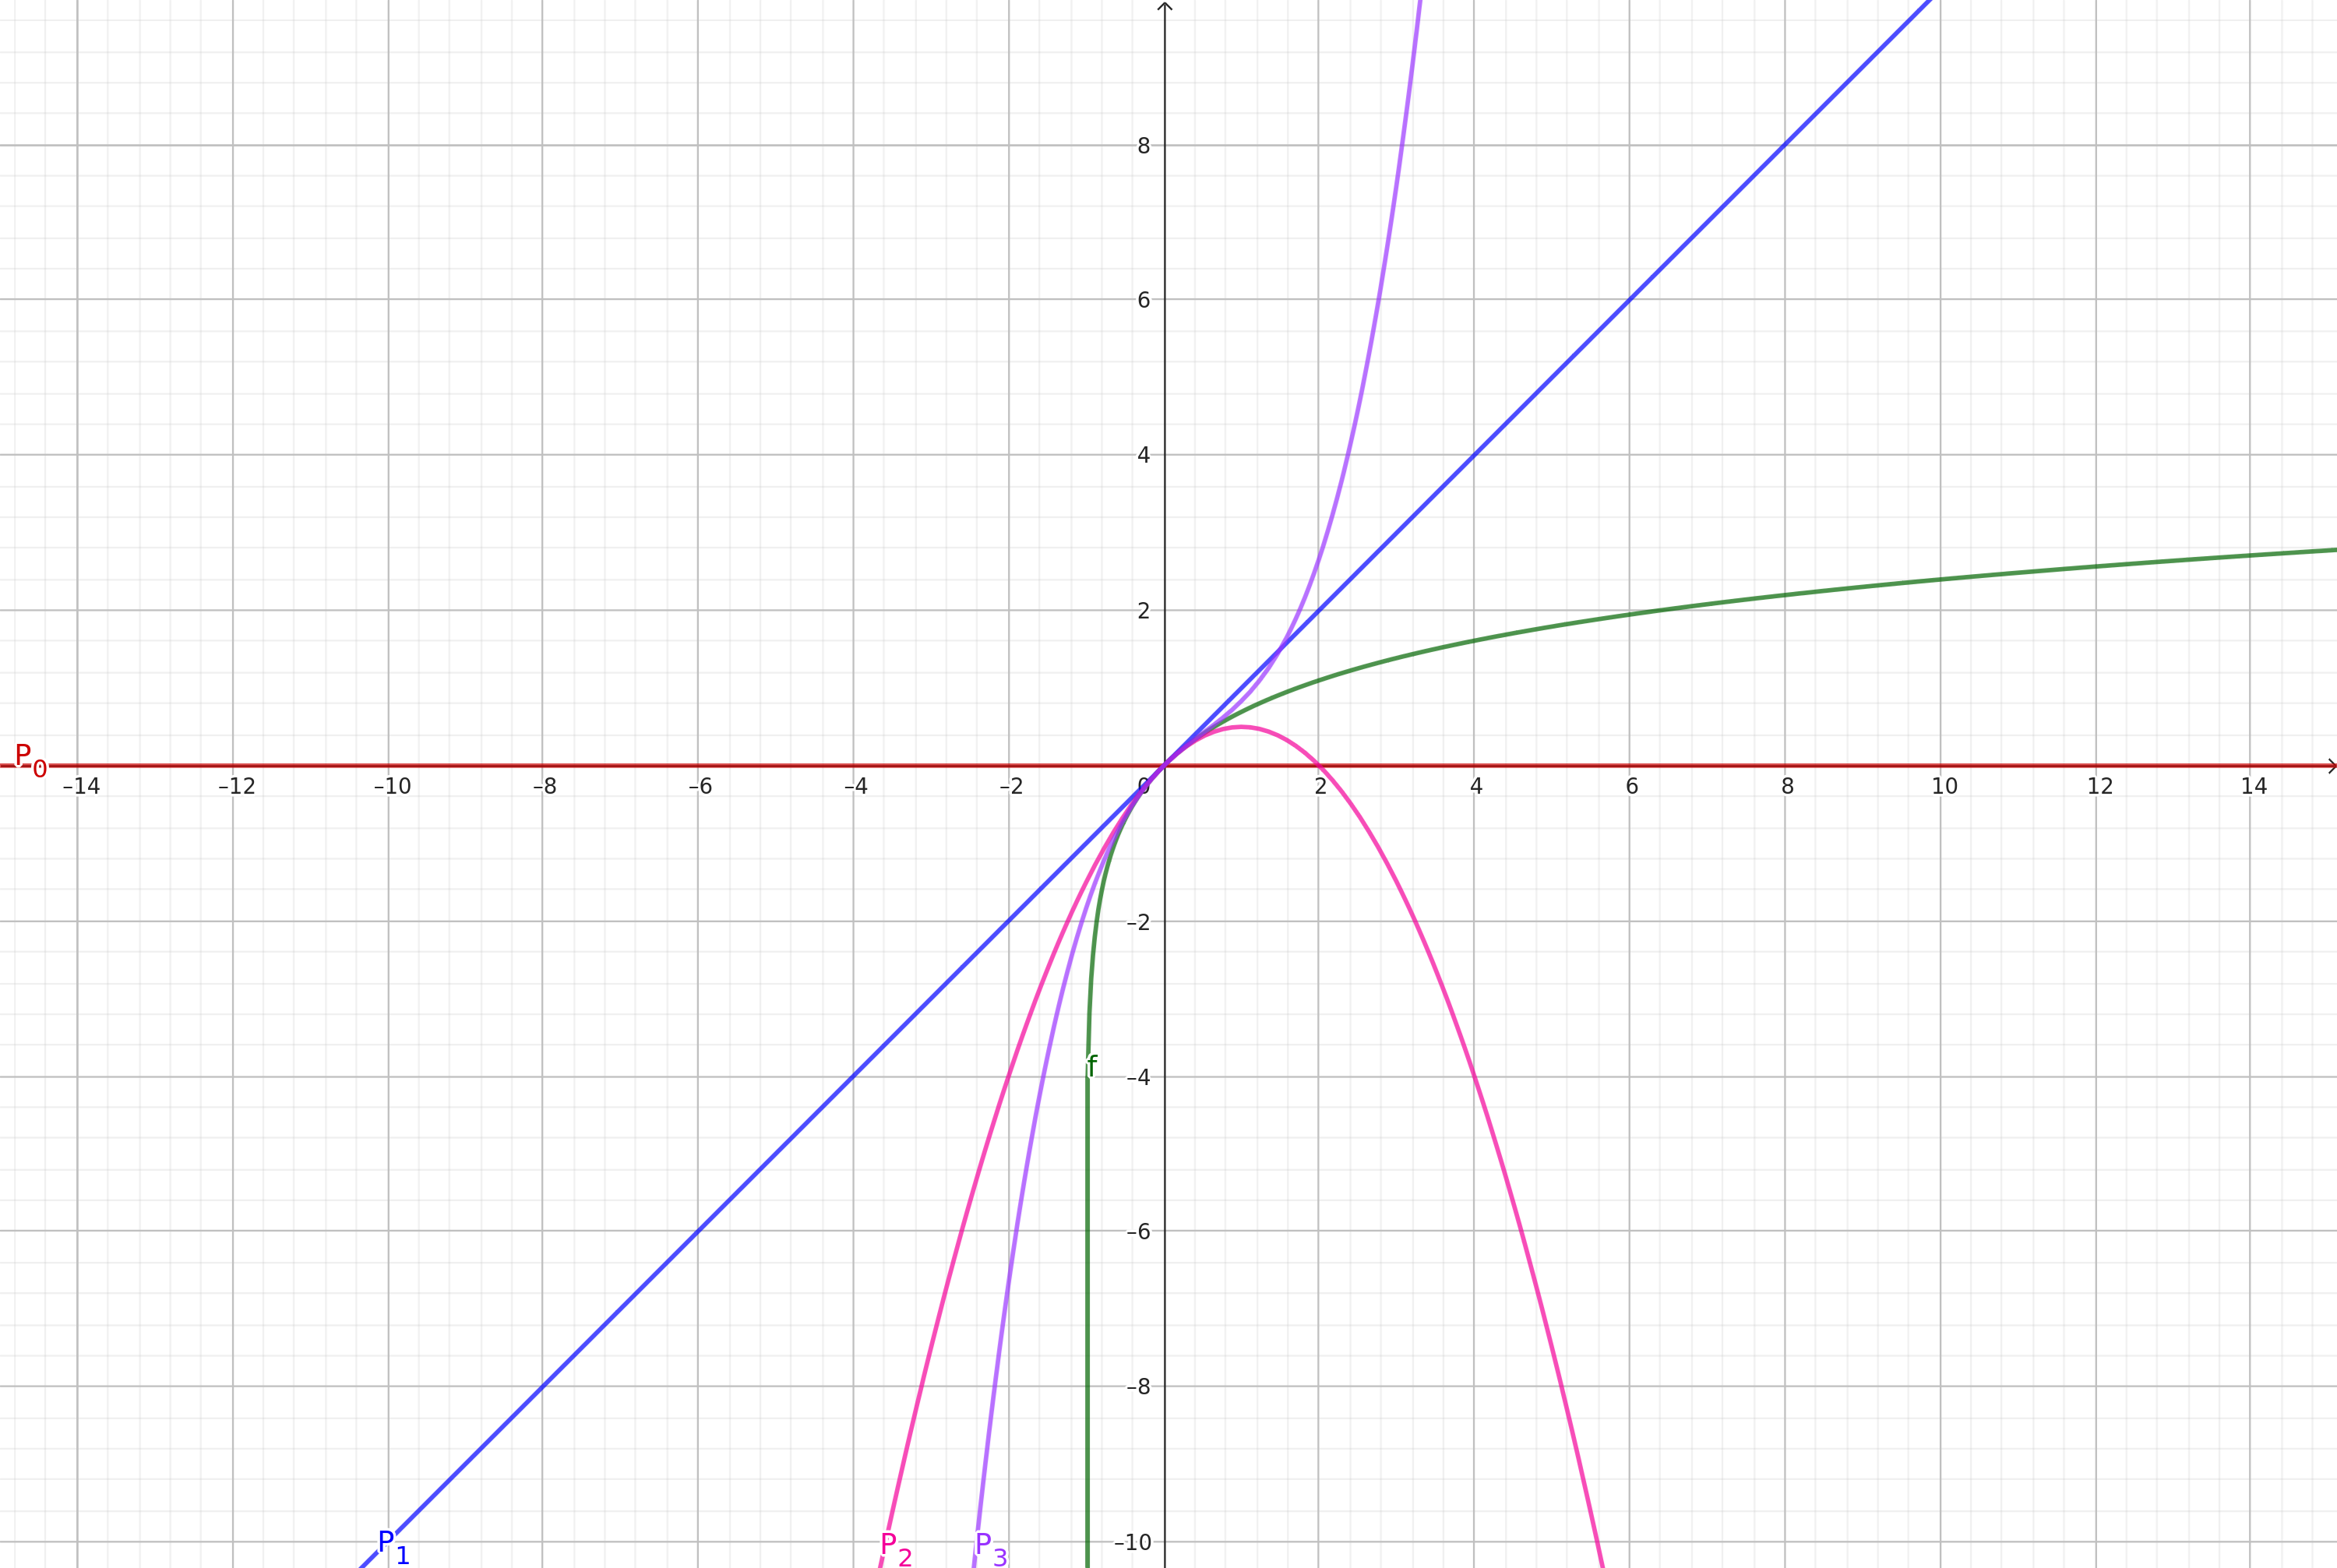
\includegraphics[height = 0.25\textheight]{recursos/polinomios/30.png}\par
    \caption*{Gráfica de la función y los Polinomios}
    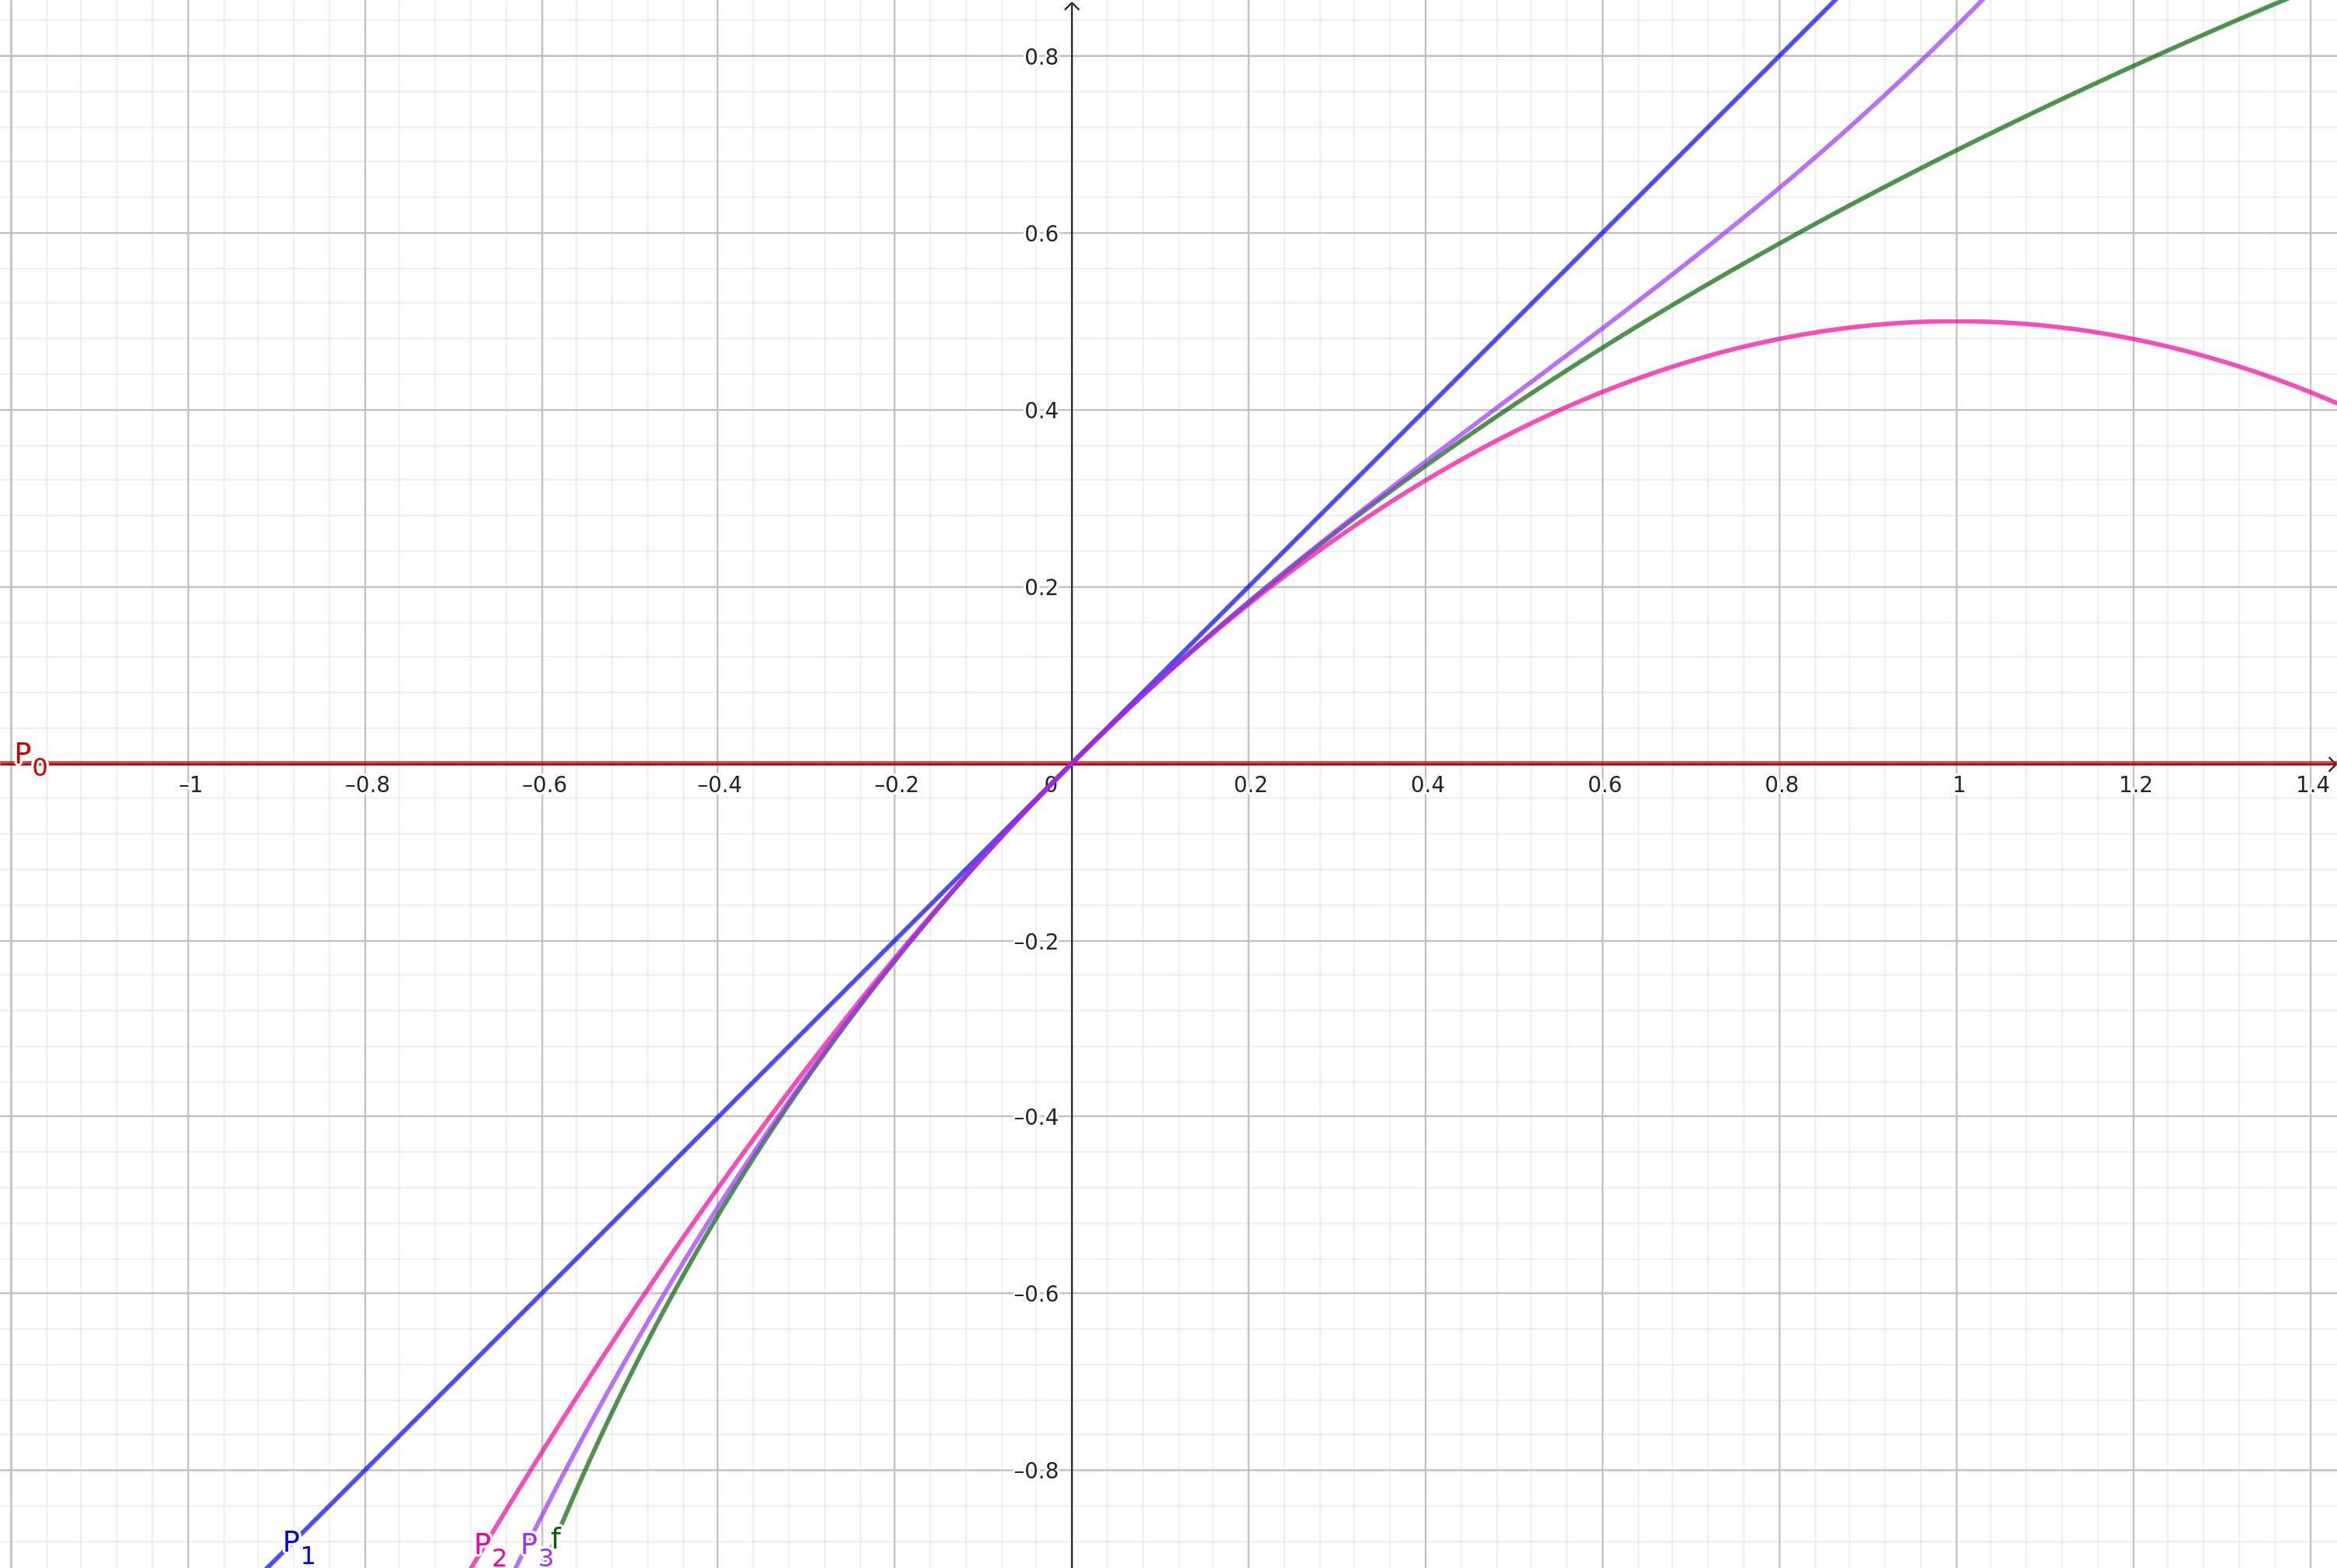
\includegraphics[height = 0.25\textheight]{recursos/polinomios/30zoom.png}\par
    \caption*{Ampliación de la Gráfica (Para notar mejor la aproximación realizada)}
    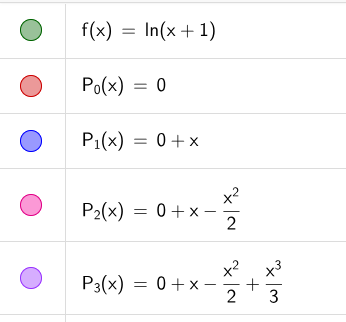
\includegraphics[height = 0.25\textheight]{recursos/polinomios/30Leyenda.png}\par
    \caption*{Simbología}
\end{figure*}